%%
% Template for Assignment Reports
% 
%

\documentclass{article}

\usepackage{fancyhdr} % Required for custom headers
\usepackage{lastpage} % Required to determine the last page for the footer
\usepackage{extramarks} % Required for headers and footers
\usepackage{graphicx,color}
\usepackage{anysize}
\usepackage{amsmath}
\usepackage{natbib}
\usepackage{caption}
\usepackage{hyperref}
\usepackage{listings}
\usepackage{float}
\usepackage{lipsum}  
\usepackage{xcolor}

% Margins
%\topmargin=-0.45in
%\evensidemargin=0in
%\oddsidemargin=0in
\textwidth=6.5in
%\textheight=9.0in
%\headsep=0.25in 

\linespread{1.0} % Line spacing

\definecolor{codegreen}{rgb}{0,0.6,0}
\definecolor{codegray}{rgb}{0.5,0.5,0.5}
\definecolor{codepurple}{rgb}{0.58,0,0.82}
\definecolor{backcolour}{rgb}{0.95,0.95,0.92}

\lstdefinestyle{mystyle}{
    backgroundcolor=\color{backcolour},   
    commentstyle=\color{codegreen},
    keywordstyle=\color{magenta},
    numberstyle=\tiny\color{codegray},
    stringstyle=\color{codepurple},
    basicstyle=\ttfamily\footnotesize,
    breakatwhitespace=false,         
    breaklines=true,                 
    captionpos=b,                    
    keepspaces=true,                 
    numbers=left,                    
    numbersep=5pt,                  
    showspaces=false,                
    showstringspaces=false,
    showtabs=false,                  
    tabsize=2
}

\lstset{style=mystyle}

%%------------------------------------------------
%% Image and Listing code
%%------------------------------------------------
%%sw \includecode{caption for table of listings}{caption for reader}{filename}
\newcommand{\includecode}[3]{\lstinputlisting[float,floatplacement=H, caption={[#1]#2}, captionpos=b, frame=single]{#3}}


%%sw \includescalefigure{label}{short caption}{long caption}{scale}{filename}
\newcommand{\includescalefigure}[5]{
\begin{figure}[htb]
\centering
\includegraphics[width=#4\linewidth]{#5}
\captionsetup{width=.8\linewidth} 
\caption[#2]{#3}
\label{#1}
\end{figure}
}

%%sw \includefigure{label}{short caption}{long caption}{filename}
\newcommand{\includefigure}[4]{
\begin{figure}[htb]
\centering
\includegraphics{#4}
\captionsetup{width=.8\linewidth} 
\caption[#2]{#3}
\label{#1}
\end{figure}
}




%%------------------------------------------------
%% Parameters
%%------------------------------------------------
% Set up the header and footer
\pagestyle{fancy}
\lhead{\authorName} % Top left header
\chead{\moduleCode\ - \assignmentTitle} % Top center header
\rhead{\firstxmark} % Top right header
\lfoot{\lastxmark} % Bottom left footer
\cfoot{} % Bottom center footer
\rfoot{Page\ \thepage\ of\ \pageref{LastPage}} % Bottom right footer
\renewcommand\headrulewidth{0.4pt} % Size of the header rule
\renewcommand\footrulewidth{0.4pt} % Size of the footer rule
\setlength\parindent{0pt} % Removes all indentation from paragraphs

\newcommand{\assignmentTitle}{Lab 1} % Assignment title
\newcommand{\moduleCode}{CSU44061} 
\newcommand{\moduleName}{Machine Learning} 
\newcommand{\authorName}{Adriana\ Hrabowych} % Your name
\newcommand{\authorID}{19304296} % Your student ID
\newcommand{\reportDate}{\printDate}

%%------------------------------------------------
%%	Title Page
%%------------------------------------------------
\title{
\vspace{-1in}
\begin{figure}[!ht]
\flushleft

\includegraphics[width=0.4\linewidth]{reduced-trinity.png}
\end{figure}
\vspace{-0.5cm}
\hrulefill \\
\vspace{0.5cm}
\textmd{\textbf{\moduleCode\ \moduleName}}\\
\textmd{\textbf{\assignmentTitle}}\\
\vspace{0.5cm}
\hrulefill \\
}

\author{\textbf{\authorName,\ \authorID}}

\date{\today}



%%------------------------------------------------
%% Document
%%------------------------------------------------
\begin{document}
\lstset{language=Java, captionpos=b, frame=single, keywordstyle=\color{black}\bfseries, stringstyle=\ttfamily}
\captionsetup{width=.8\linewidth} 

\maketitle


%%------------------------------------------------
\section{Part A: Logistic Regression Classifier}
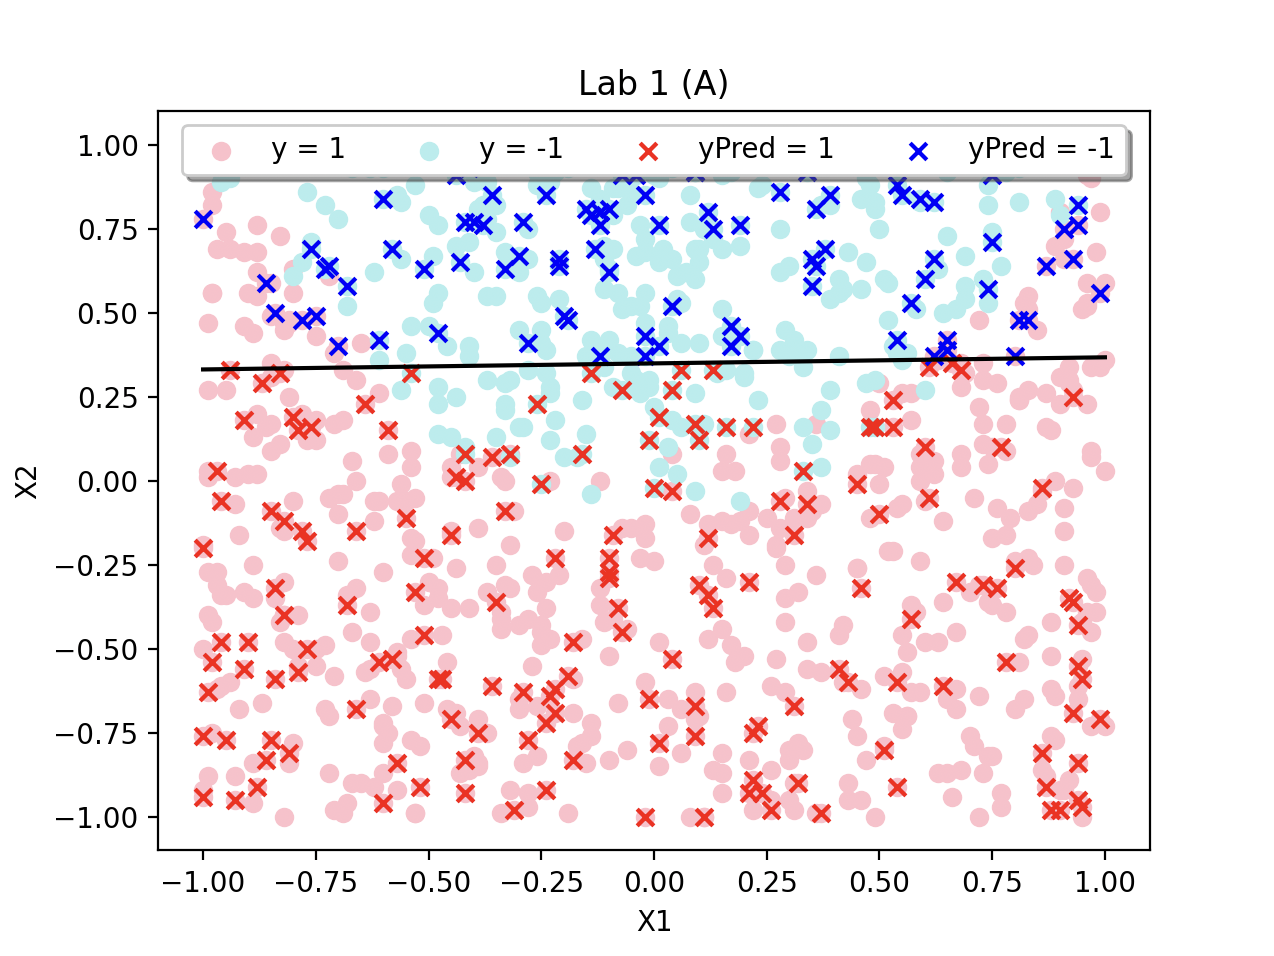
\includegraphics[width=\linewidth]{pA.png}
\captionof{figure}{A scatter plot graph visualizing part A of the lab. Dataset used is id:13-13--13}

\subsection{A(i)}
In A(i) the raw data is read in and then visualized on the graph seen in figure one using circular markers. Each data point is placed depending on the value of its two features, with the X-axis corresponding to X1 and the Y-axis corresponding to X2. The color of the marker depends on the target value y, if the marker is red then y=1 and if blue then y=-1.

\subsection{A(ii)}
The data is then randomly split with 25\% being used for testing our models and 75\% to be used for training our models. The ratio 25-75 was chosen as it is the default for the sklearn method and is typical for test-train splits.

A logistic regression model is then trained using the training data. The default sklearn parameters are used to define this model as they follow the usual standard for the parameters. The equation the model uses to predict the y values is sign($\theta^{T}x$), where $\theta^{T}x$ = $\theta_0 + \theta_1x_1 + \theta_2x_2$. The x's represent the two input features X1 and X2 while the thetas, bar theta 0 which is the intercept, are the parameters the model defines once trained. 

Feature X2 has the greater influence on the prediction as when looking at the absolute values of the models coefficients, X2's is larger meaning it skews the prediction more. Each time the code is run the values change slightly as the data is split differently, but in one example the coefficients were:

\begin{center} $\theta_1 = 0.1148 \quad \quad  \quad \theta_2 = -4.5772  \quad \quad  \quad intercept =  1.5772$\end{center}

From this we can see that X2's coefficient has much more influence and skews the results towards being negative and X1's coefficient, while small, skews the data positively.

\subsection{A(iii)}
The model is then given the test features and outputs the predicted y values. These predicted y's are then plotted as seen in figure one using x markers. The color of these markers have the same meaning as the raw data colors, just brighter for easier legibility. In addition a decision boundary is added to the graph in black. 

The decision boundary was calculated using the intercept and the feature coefficients. This information was fitted to a linear equation ax + (intercept / $\theta_2$) = 0. The intercept was divided by $\theta_2$ in order to translate the intercept from being for the model itself to reflecting the decision boundaries intercept. The slope of the line, a, was calculated with the equation $-\theta_1 / \theta_2$. 

\subsection{A(iii)}
The accuracy of the model is not perfect, the mean squared error of the model with these parameters equaled 0.528. As seen in figure one, the raw y values and the predicted y values differ quite dramatically. Though the general area of the red x's and blue x's match where the corresponding circles are the shape of the division between the two differs. Whereas the raw data has a curved division, the predictions have a straight line division. 

%%------------------------------------------------
\section{Part B: Linear SVM Classifier}
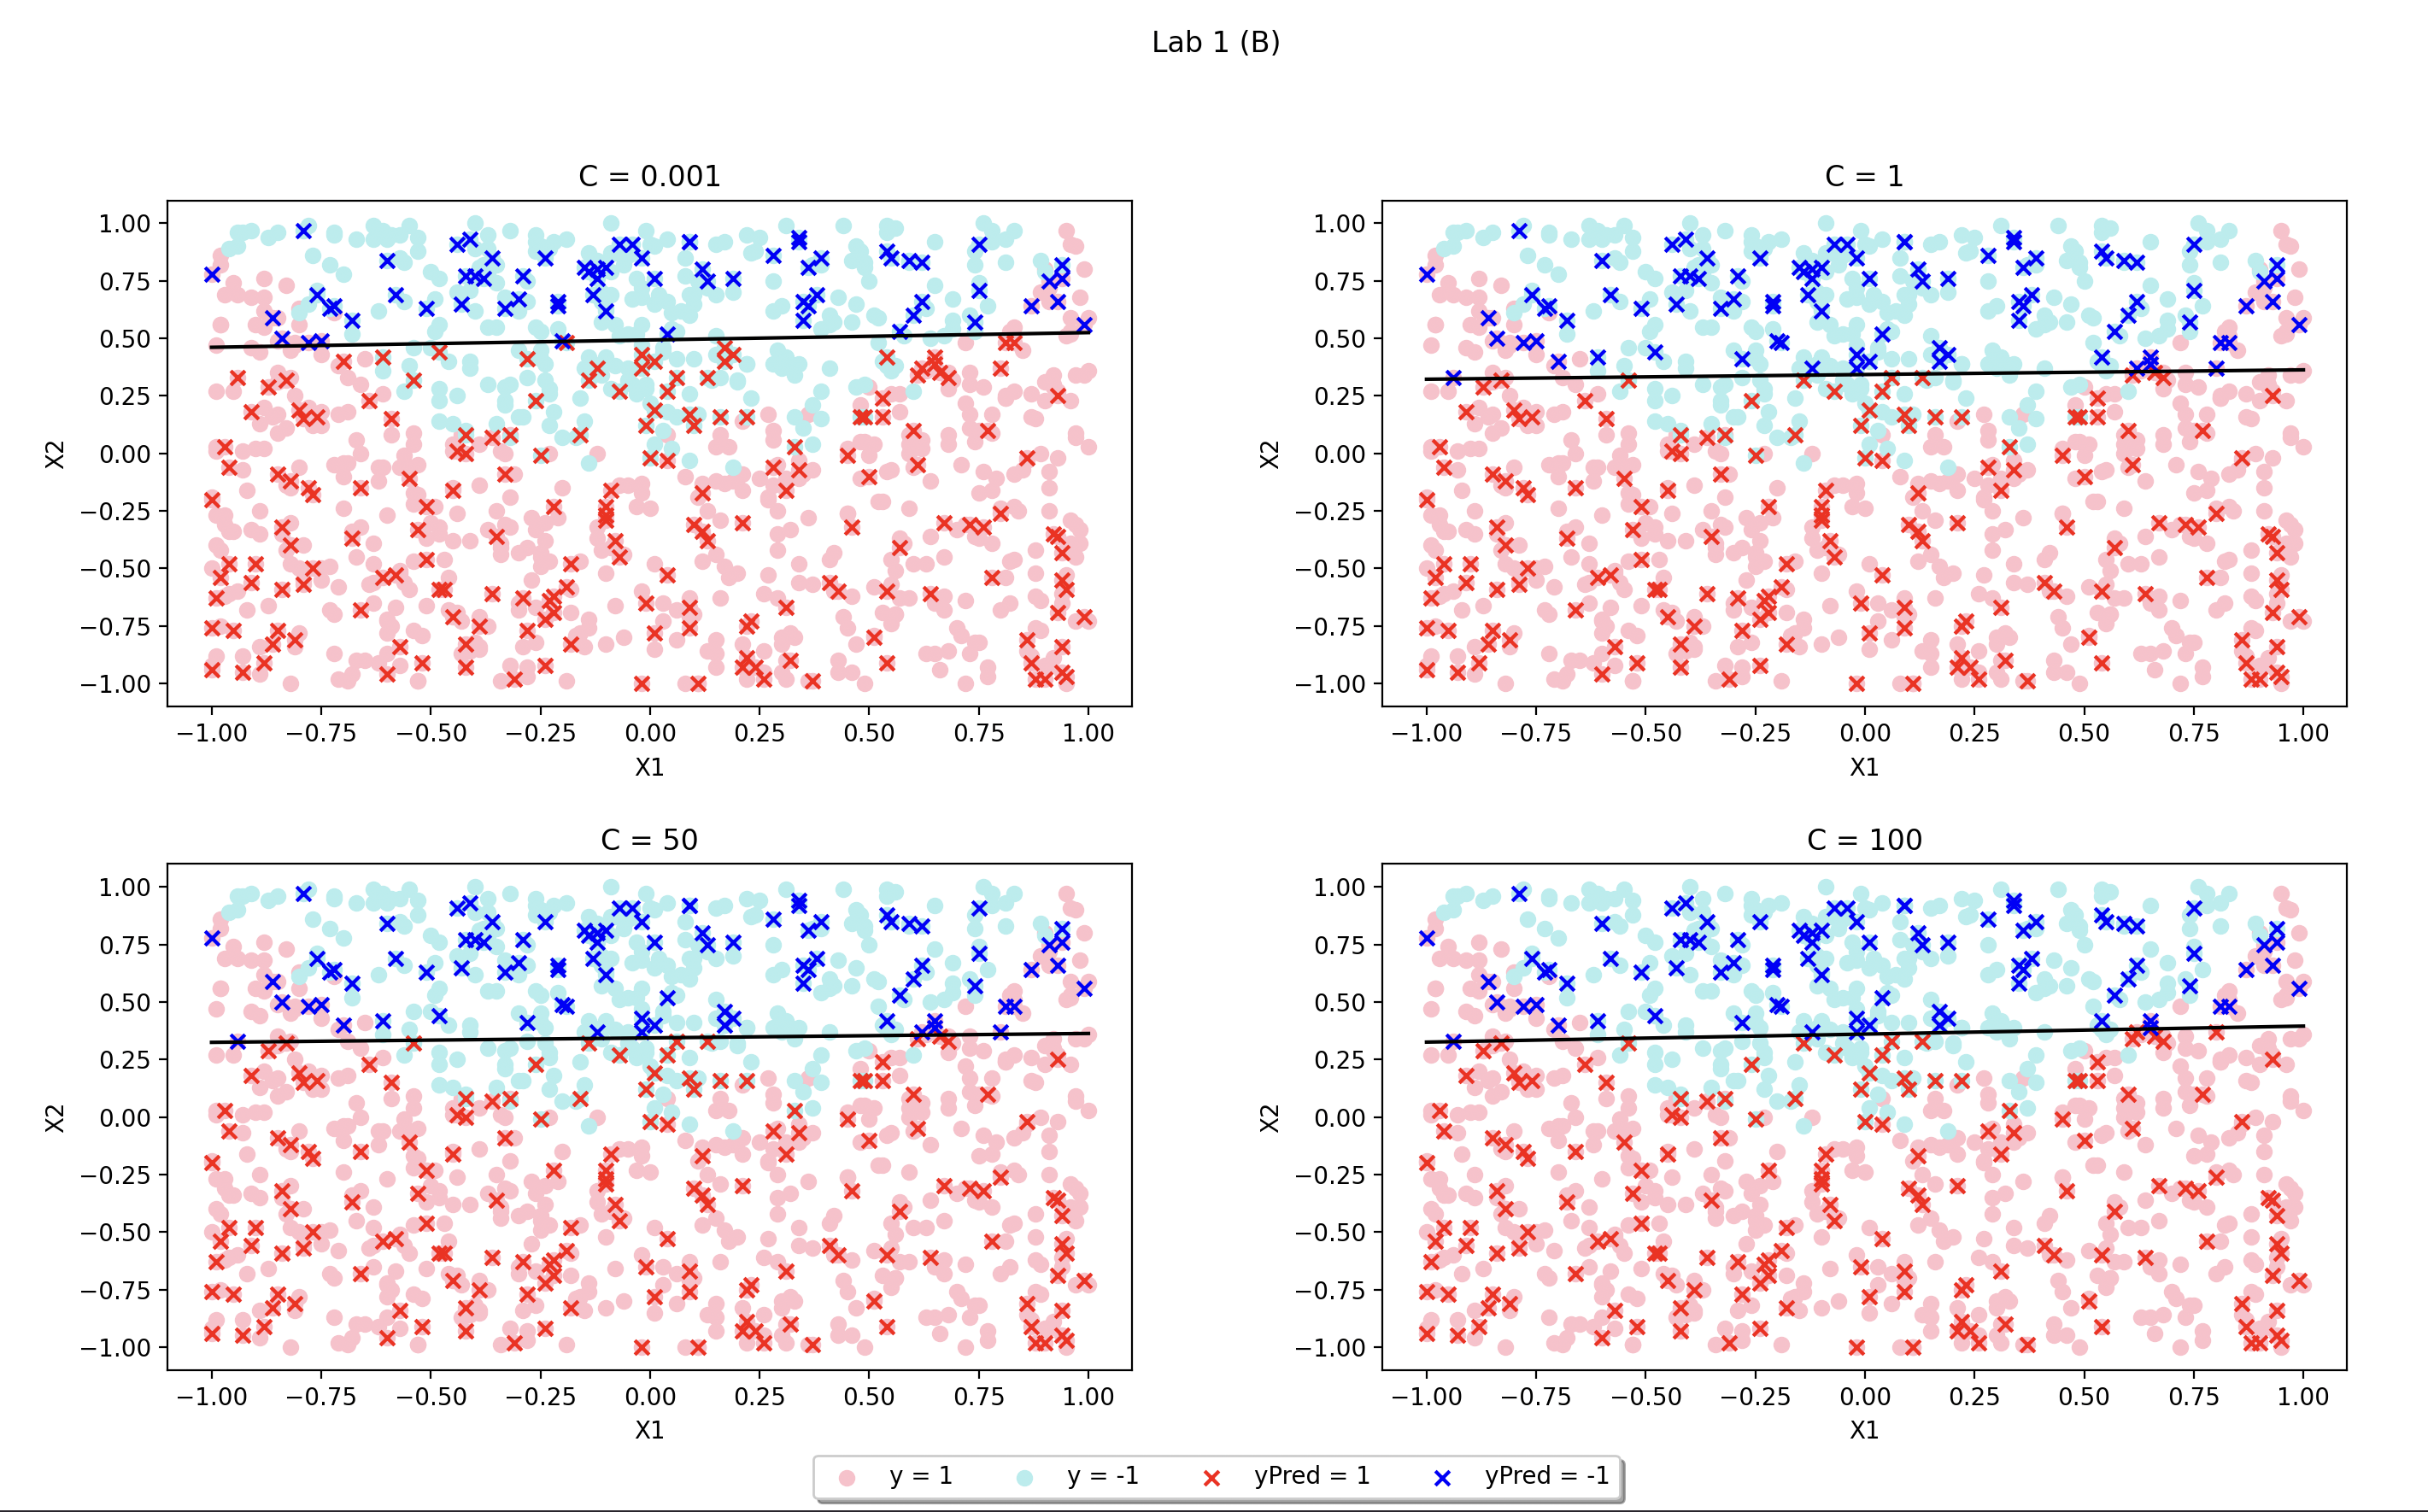
\includegraphics[width=\linewidth]{pB.png}
\captionof{figure}{A figure containing 4 scatter plots visualizing part B of the lab. Dataset used is id:13-13--13}

\subsection{B(i)}
In part B(i), four SVM Classifiers were trained on the same test and training data as each other and the model in the previous part. The equation these models uses to predict the y values is sign($\theta^{T}x$), where $\theta^{T}x$ = $\theta_0 + \theta_1x_1 + \theta_2x_2$. The x's represent the two input features X1 and X2 while the $\theta_1 and \theta_2$ are the parameters the model defines once trained. $\theta_0$ represents the model intercept.

The only difference between the four models is that each one has a different value for C, either 0.001, 1, 50, and 100. One run of the code gave the following coefficients and intercepts:
\begin{center} C= 0.001: $\theta_1 = 0.0084 \quad \quad  \quad \theta_2 = -0.3906  \quad \quad  \quad intercept =  0.1806$\end{center}
\begin{center} C= 1: $\theta_1 = 0.0478 \quad \quad  \quad \theta_2 = -1.7132  \quad \quad  \quad intercept =  0.5753$\end{center}
\begin{center} C= 50: $\theta_1 = 0.0394 \quad \quad  \quad \theta_2 = -1.7238  \quad \quad  \quad intercept =  0.5898$\end{center}
\begin{center} C= 100: $\theta_1 = 0.0638 \quad \quad  \quad \theta_2 = -1.6036  \quad \quad  \quad intercept =  0.5729$\end{center}

\subsection{B(ii)}
Each model is plotted on its own graph for legibility. Each graph has the same raw data, plotted in the same way as in part A. The predicted Y values are then again, for each model and graph, plotted using red and blue x markers. Red signifies Y = 1 and blue signifies Y = -1. A decision boundary is also plotted for each model using the same equation as in part A.

\subsection{B(iii)}
In SVM models, C defines the priority of minimizing errors during training. A low C value allows a larger margin while a high C value has a lower tolerance for training error. The trend for the model coefficients is that the larger C becomes, the larger $\theta_1, \theta_2$, and the intercept become. This results in differences in the accuracy of predictions, with these coefficients and parameters the mean squared error of each model is given as C=0.001 has an accuracy of 0.64, C=1 has one of 0.528, C=50 has 0.528, and C=100 has 0.544.

From these accuracies it is clear the importance of choosing a good C value for a model, having a C too small and having a C too big can ruin the accuracy of a model. Finding the C that balances the margins and tolerance for training errors is an important step in defining your model. For this example a C between 1 and 50 provided the best accuracy.

\subsection{B(iv)}
The most noticeable difference between the SVM Classifiers and the Logistic Regression Classifier is the size of the coefficients and intercepts. The intercept for our Logistic Regression Classifier was 1.5772 while the SVM models has intercepts ranging between 0.1 and 0.6. The former is nearly three times the size of the latter, which is a large gap. The coefficients for our Logistic Regression Classifier were 0.1148 and -4.5772 for X1 and X2 respectively. While the SVM models had coefficients for X1 being ranging between ~0.008 and 0.04 and for X2 being between -0.3 and -1.7. Once again the Logistic Regression model had larger numbers than the SVM models.

Though these differences did not result in a large change in accuracy, the Logistic Regression model has an mean squared error value of 0.528 which is the same as the SVM models with C=1 and C=50. The other two models are not that far away either with error of C=0.001 being 0.64 and C=100 being 0.544.

%%------------------------------------------------
\section{Part C: Logistic Regressor with Four Features}
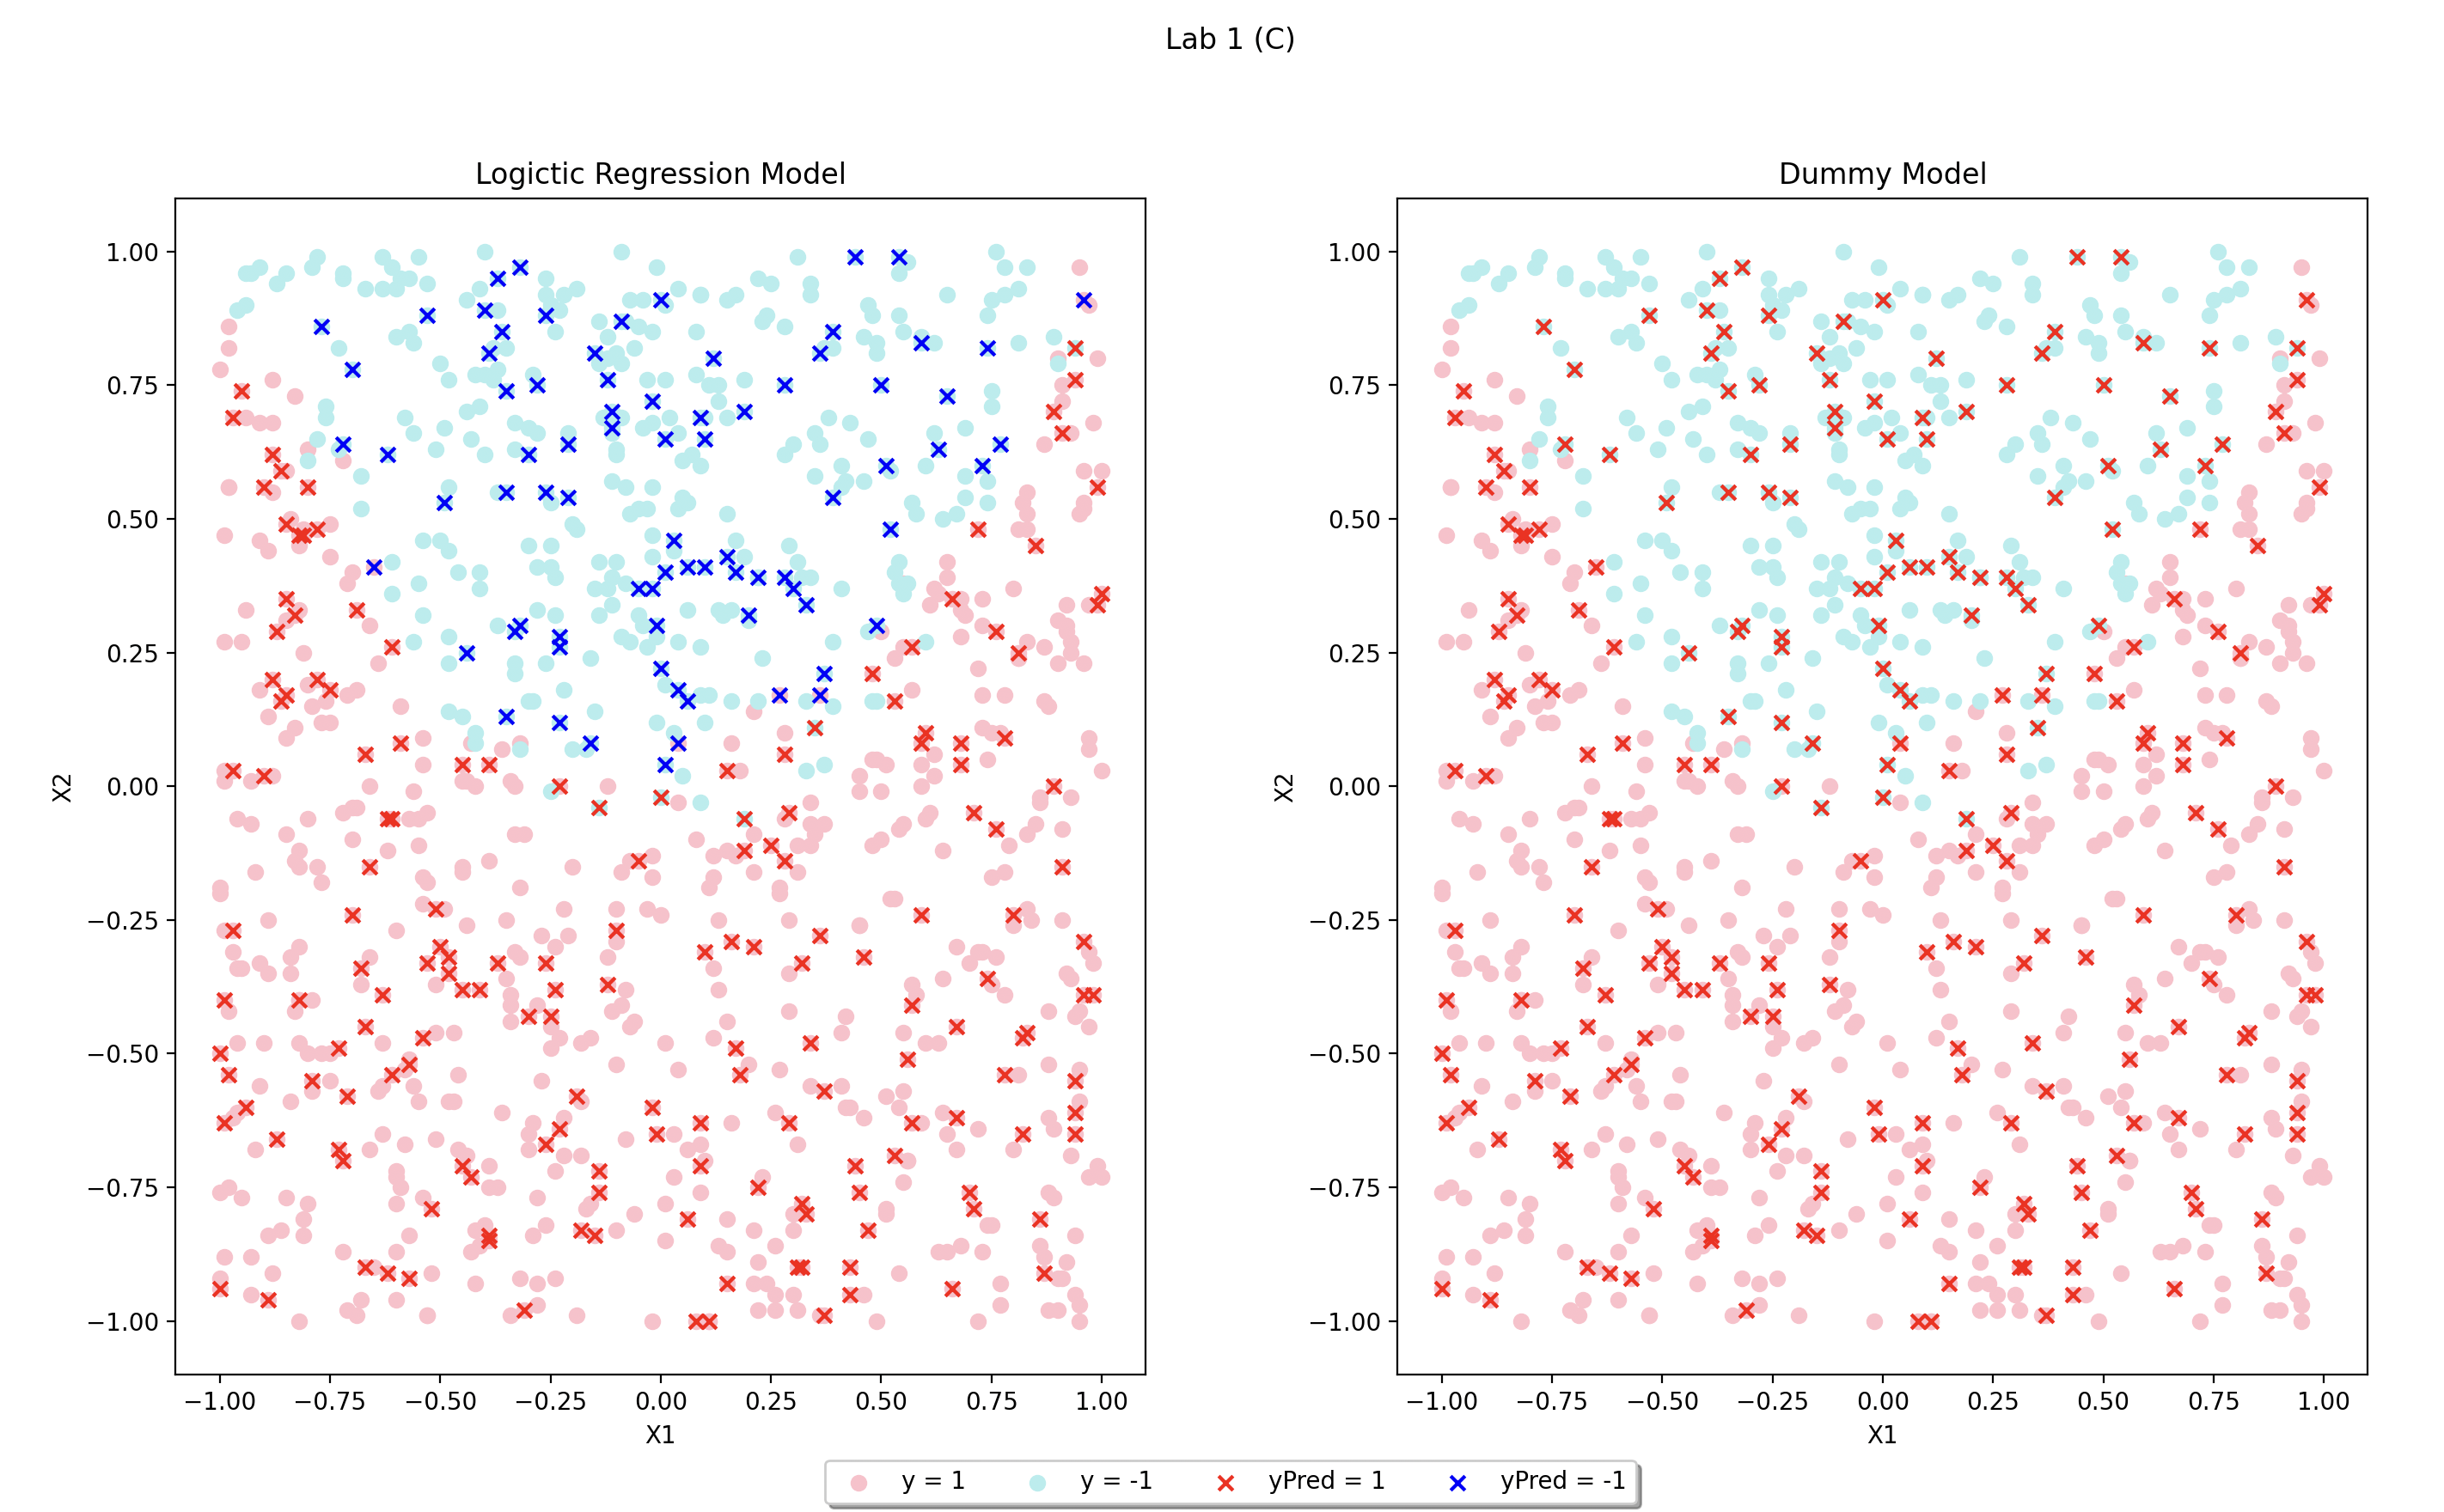
\includegraphics[width=\linewidth]{pC.png}
\captionof{figure}{A figure containing 2 scatter plots visualizing part C of the lab. Dataset used is id:13-13--13}
\subsection{C(i)}
We create the two additional features by squaring both X1 and X2 and giving them to the model in addition to the original X1 and X2. The equation this model now uses to predict the y values is $sign(\theta^{T}x$), where $\theta^{T}x$ = $\theta_0 + \theta_1x_1 + \theta_2x_2 + \theta_3x_1^2 + \theta_4x_2^2$. $\theta_0$ represents the intercept, and the other thetas are the coefficients for their corresponding X's. 

In one run of the code the coefficients for the data were $\theta_0 = 0.1961, \theta_1 = 0.1584, \theta_2 = -5.9691, \theta_3 = 6.163, $and $\theta_4 = -0.7811.$

\subsection{C(ii)}
In figure 3, the graph on the left is a visualization of this 4-feature Logistic Regression model. Each data point is placed depending on the value of the first two features, with the X-axis corresponding to X1 and the Y-axis corresponding to X2. The color of the marker depends on the target value y, if the marker is red then y=1 and if blue then y=-1.

The predictions made by this model are much more accurate than the ones in part A and B, the boundary between the red and blue predicted value are now a curve like in the raw data. This is due to the face that the two additional features added changed the decision boundary from a linear equation to a quadratic equation. The mean squared error given by this model was 0.096, which is incredibly low compared to the 2-feature Logistic Regression and SVM models.

\subsection{C(iii)}
In figure 3, the graph on the left is a visualization of a 4-feature 'Dummy' model. Each data point is placed depending on the value of the first two features, with the X-axis corresponding to X1 and the Y-axis corresponding to X2. The color of the marker depends on the target value y, if the marker is red then y=1 and if blue then y=-1.

This dummy model always predicts whatever the most common y-value was during training, which in this case was y=1 so every predicted mark is red. The mean squared error for this baseline is 1.472, which is much worse than the four-feature Logistic Regression model and every other model we've had in this lab. This is too be expected however as the model is very simplistic.

\section{Appendix}
\lstinputlisting[language=Python]{main.py}
\end{document}
\end{document}

